\scanpage{153}
% archive foliation: 152
\figure{\begin{tikzpicture}[x=.65cm,y=.65cm]
\draw (0,6)--(2,8); \draw (.7,7.8)--(1.3,5.2); \draw (1.2,7.8)--(2.35,6.1);
\draw (.7,5.9)--(3.2,4.5); \draw (1.7,5.7)--(1.7,4.35); \draw (2.25,5.55)--(2.1,4.1);
\node at (3.5,4.5) {$g$};
\draw (-.1,2.3)--(1.15,4); \draw (.2,4.25)--(.55,1.7); \draw (.6,4.05)..controls (1.15,3.9)..(1.7,2.7);
\draw (.05,2.05)--(1.7,1.1); \draw (.7,2.1)--(1.3,.25); \draw (1.25,2.1)--(.9,.65); \fill (1.05,1.55) circle (2pt);
\draw (3,1)--(4.6,2.6); \draw (3.15,2.4)--(3.6,-.1); \draw (4,2.7)..controls (4.2,1.5)..(4.85,.7);
\draw (3.2,.6)--(5.8,-1.15); \draw (4.15,.25)--(4,-1); \draw (4.7,.05)--(4.5,-1.3); \draw (5.35,-.1)--(4.95,-2.65);
\node at (5.8,.05) {$g''$}; \node at (6.1,-1.2) {$g'$};
\node at (9,-.3) {$g'+g''=g\quad(g'+g''>0)$};
\draw (11,2)--(13,3.5); \draw (11.3,3.2)..controls (11.6,1.6)..(12.1,.9); \draw (12.65,3.65)..controls (12.9,2.7)..(13.5,2.05);
\draw (11.2,1.5)--(14.2,.65); \draw (11.45,1.85)--(11,.1);
\draw (12.55,1.6)--(12.5,.1); \draw (13.05,1.4)--(13,.0); \draw (13.55,1.2)--(13.65,-.2);
\node at (14.7,.65) {$\deleted{\unsure{g}}g'=0$}; \node at (17,.55) {$(g=0$};
\end{tikzpicture}}
\[
\sum_{g_i\unsure{\geq|>}1}(3g_i-3+\nu_i\deleted{\unsure{0}})
+\sum_{g_i=1}\underbrace{(1+\nu_i-1)}_{3g_i-3+\nu_i}
+\sum_{\substack{g_i=0\\\nu_i\unsure{>|\geq}3}}
\deleted{\text{\unsure{sauf les}\illegible{1}}}\underset{3g_i-3+\nu_i}{\nu_i-3}
\]
$\nu_i=$ nb des pts \deleted{\unsure{multiples}}\inserted{\unsure{marqués}} sur $C_i$
\[
3\sum g_i-3c_0+\sum\nu_i+\overset{\lambda}{\boxed{\sum_{\substack{g_i=0\\\nu_i\leq2}}3-\nu_i}}
\]
$\lambda=$ nb des courbes $C_i$ de genre $0$, avec $\nu_i=2$ (\unsure{minimum})
\figure{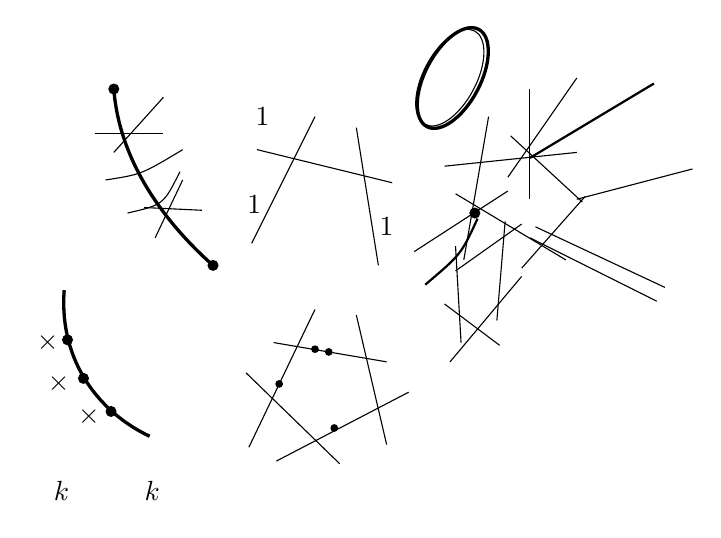
\begin{tikzpicture}[x=.7cm,y=.7cm]
\draw[very thick] (0,6)..controls (.1,4.7) and (.9,3.6)..(1.8,2.8); \fill (0,6) circle (2pt); \fill (1.8,2.8) circle (2pt);
\draw (-.35,5.2)--(.9,5.2); \draw (0,4.85)--(.9,5.85); \draw (-.15,4.35)..controls (.5,4.45)..(1.25,4.9);
\draw (.25,3.75)..controls (.9,3.9)..(1.2,4.5); \draw (.55,3.85)--(1.6,3.8); \draw (.75,3.3)--(1.25,4.35);
\draw (2.6,4.9)--(5.05,4.3); \draw (2.5,3.2)--(3.65,5.5); \draw (4.4,5.3)--(4.8,2.8);
\node at (2.7,5.5) {$1$}; \node at (2.55,3.9) {$1$}; \node at (4.95,3.5) {$1$};
\draw[very thick,rotate around={-28:(6.15,6.2)}] (6.15,6.2) ellipse (.5 and 1); \draw[rotate around={-28:(6.15,6.2)}] (6.1,6.18) ellipse (.48 and .96);
\draw[very thick] (-.9,2.35)..controls (-1,1) and (-.2,.1)..(.65,-.3);
\fill (-.84,1.45) circle (2pt);\fill (-.55,.75) circle (2pt);\fill (-.05,.15) circle (2pt);
\node at (-1.2,1.4) {$\times$};\node at (-1,.65) {$\times$};\node at (-.45,.05) {$\times$};
\node at (-.95,-1.3) {$k$};\node at (.7,-1.3) {$k$};
\draw (2.9,1.4)--(4.95,1.05);\draw (3.65,2)--(2.45,-.5);\draw (4.4,1.9)--(4.95,-.45);\draw (2.4,.85)--(4.1,-.8);\draw (2.95,-.75)--(5.35,.5);
\fill (3.65,1.28) circle (1.4pt);\fill (3.9,1.23) circle (1.4pt);\fill (3,.65) circle (1.4pt);\fill (4,-.15) circle (1.4pt);
\draw (6,4.6)--(8.4,4.85);\draw (7.55,6)--(7.55,4);\draw (7.15,4.4)--(8.4,6.2);\draw[thick] (7.55,4.75)--(9.8,6.1);\draw (7.2,5.15)--(8.5,3.95);\draw (8.4,4)--(10.5,4.55);
\draw (6.8,5.5)--(6.35,2.9);\draw (5.45,3.05)--(7.15,4.15);\draw[thick] (5.65,2.45)..controls (6.3,3)..(6.6,3.65);\draw (6.2,4.1)--(8.2,2.9);\fill (6.55,3.75) circle (2pt);
\draw (6.2,3.15)--(6.3,1.4);\draw (6.2,2.7)--(7.4,3.55);\draw (7.1,3.6)--(6.95,1.8);\draw (6,2.1)--(7,1.35);\draw (6.1,1.05)--(7.4,2.6);
\draw (7.55,3.3)--(9.85,2.15);\draw (7.65,3.5)--(10,2.4);\draw (7.4,2.75)--(8.55,4.05);
\end{tikzpicture}}
\margin{[ tout cycle est formé exclusivement de courbes rationnelles, et \deleted{\unsure{est de}}\inserted{un cycle} minimum est de longueur un}
\[
\sum g_i\unsure{=|\equiv}g-\rho.
\]
\margin{$\rho$: nbr des cycles combinatoires}
\[
3g-
\]

